% file: 3-1-dp/rod-cutting-opt.tex

\documentclass[tikz]{standalone}

\usetikzlibrary{calc, shapes.multipart}
 
\begin{document}
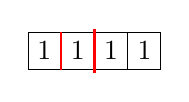
\begin{tikzpicture}[]
  \node (rod) [rectangle split, rectangle split parts = 4, draw, anchor = center, rectangle split horizontal]
    {$1$\nodepart{two}$1$\nodepart{three}$1$\nodepart{four}$1$};

  % \draw [red, thick] (rod.north) to (rod.south);
  \draw [red, thick] ($(rod.text split) + (0, -7pt)$) to ($(rod.text split) + (0, 7pt)$);
  \draw [red, thick] ($(rod.two split) + (0, -8pt)$) to ($(rod.two split) + (0, 8pt)$);
\end{tikzpicture}
\end{document}
